\chapter{Brukerveiledning}

%\section{Boligsøker}

\subsection{Filterpanel}
\subsection{Resultattabell}
\subsection{Visningspanel}
Presentasjon av data og bilder over eiendommer.
\subsection{Forespørsel}
%\section{Megler}

Pålogging
Søkepanel
Resultattabell
Outputvindu. Data bilder
Registrering og endring av ny utleier
Registrering og endring av ny bolig
Opplastning av bilder
Registrering av en ny annonse
Oprettelse av kontrakt
Sletting

\subsection{Pålogging}
\subsection{Menyer}
menyer som presenteres ved høyreklikk. 
\subsection{Søkepanel}
\subsection{Resultattabell}
\subsection{Visningspanel}
Data og presentasjon av bilder over eiendomer.
\subsection{Utleieradministrasjon}
Registrering og endring.
\subsection{Boligadministrasjon}
Registrering og endring.
\subsection{Annonser}
\subsection{Kontrakt}
\subsection{Sletting}

%LEGGER INN ALT HER I EN FIL



\section{Forord}
Programmet er delt opp i 2 hoveddeler - en del for boligsøkende, og en del for megler/
administrasjon. Disse to delene av programmet er adskilt ved hjelp av arkfaner oppe i venstre
hjørne av programmet (figur \ref{fig:bv:1}).

Vinduet for boligsøkende (figur \ref{fig:bv:1}) er i hovedsak delt opp i 4 deler, som vi går videre inn på nå.




\begin{figure}[h!]
 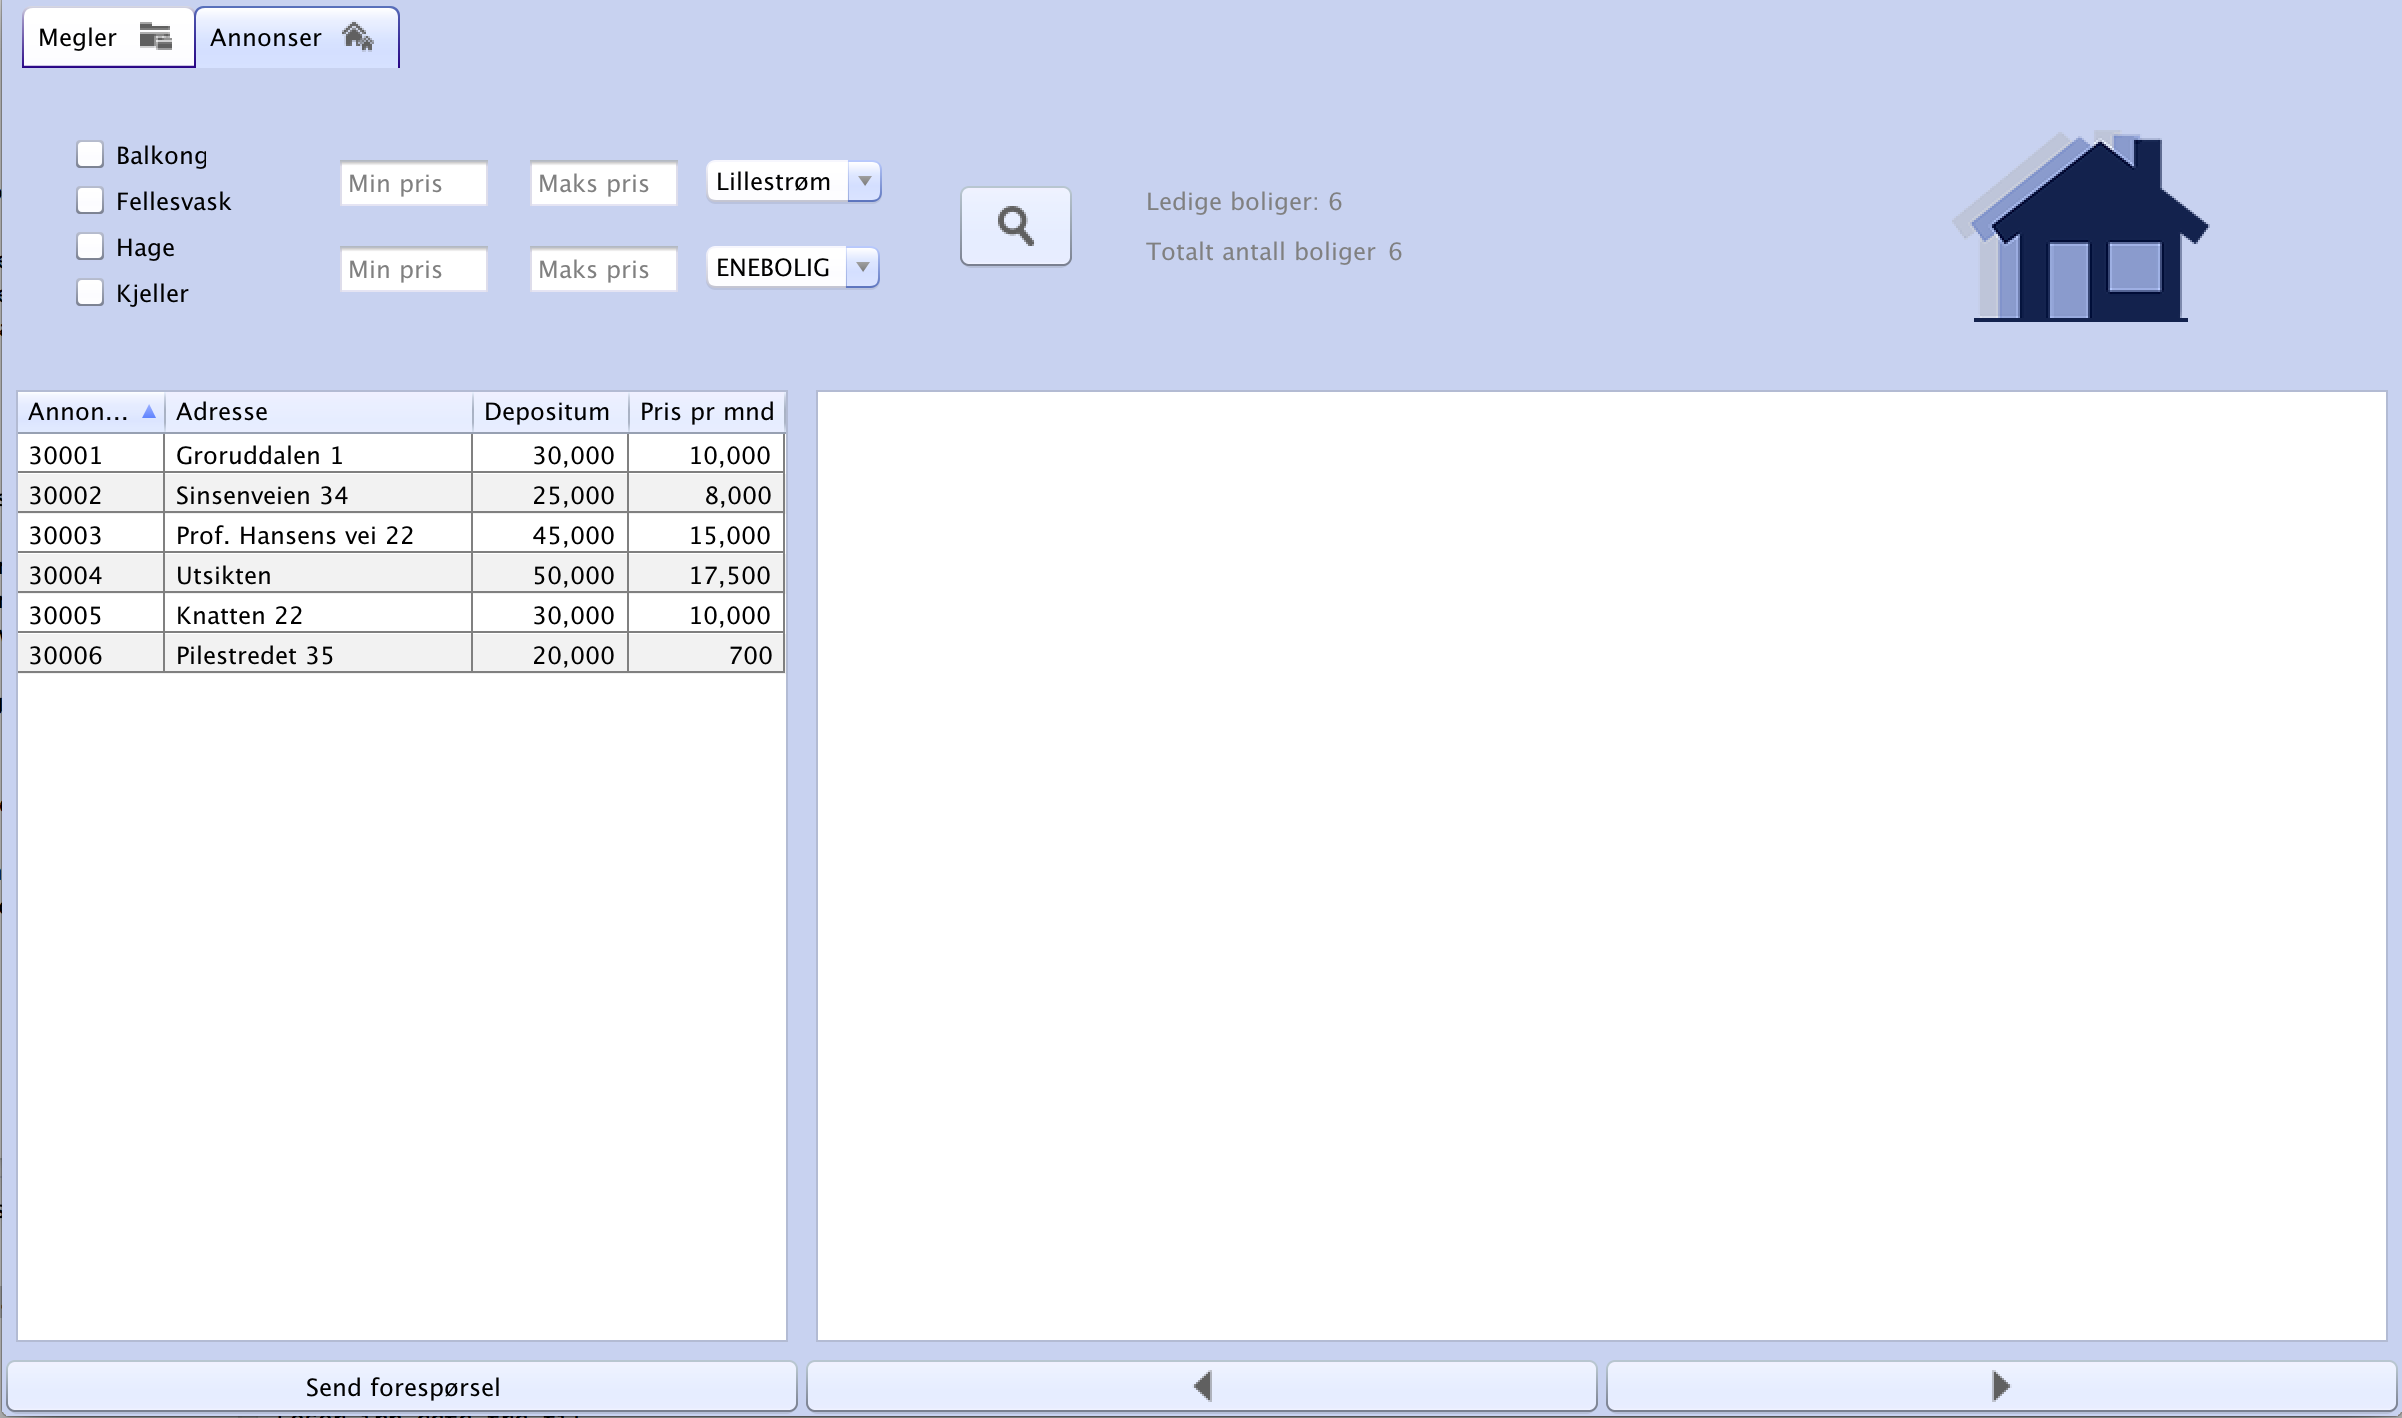
\includegraphics[width=\textwidth,height=\textheight,keepaspectratio]{./img/brukerveiledning/1.png}
 \caption{Boligsøkende.}
 \label{fig:bv:1}
\end{figure}




%//////////////////////////////////////////////

\section{Bolisøker}



\subsection{Filterpanel}

Dette er øverste del av programvinduet markert i rødt på figur \ref{fig:bv:2}. Her har en muligheten til å
legge inn ønskede søkekritierier, og søke blant tilgjengelige boliger ut ifra valgte kriterier.
En kan til enhver tid trykke på “Enter” knappen for å gjøre et søk ut ifra valgte kriterier, eller ved å
enkelt og greit trykke på søk-knappen.

Merk at tilgjengelige stedsnavn i dropdown menyen, vil kun vise stedsnavn for steder det er
registrert boliger for. Finner du ikke stedsnavnet ditt i denne listen, så er det heller ingen
tilgjengelige boliger i det aktuelle området.



\begin{figure}[h!]
 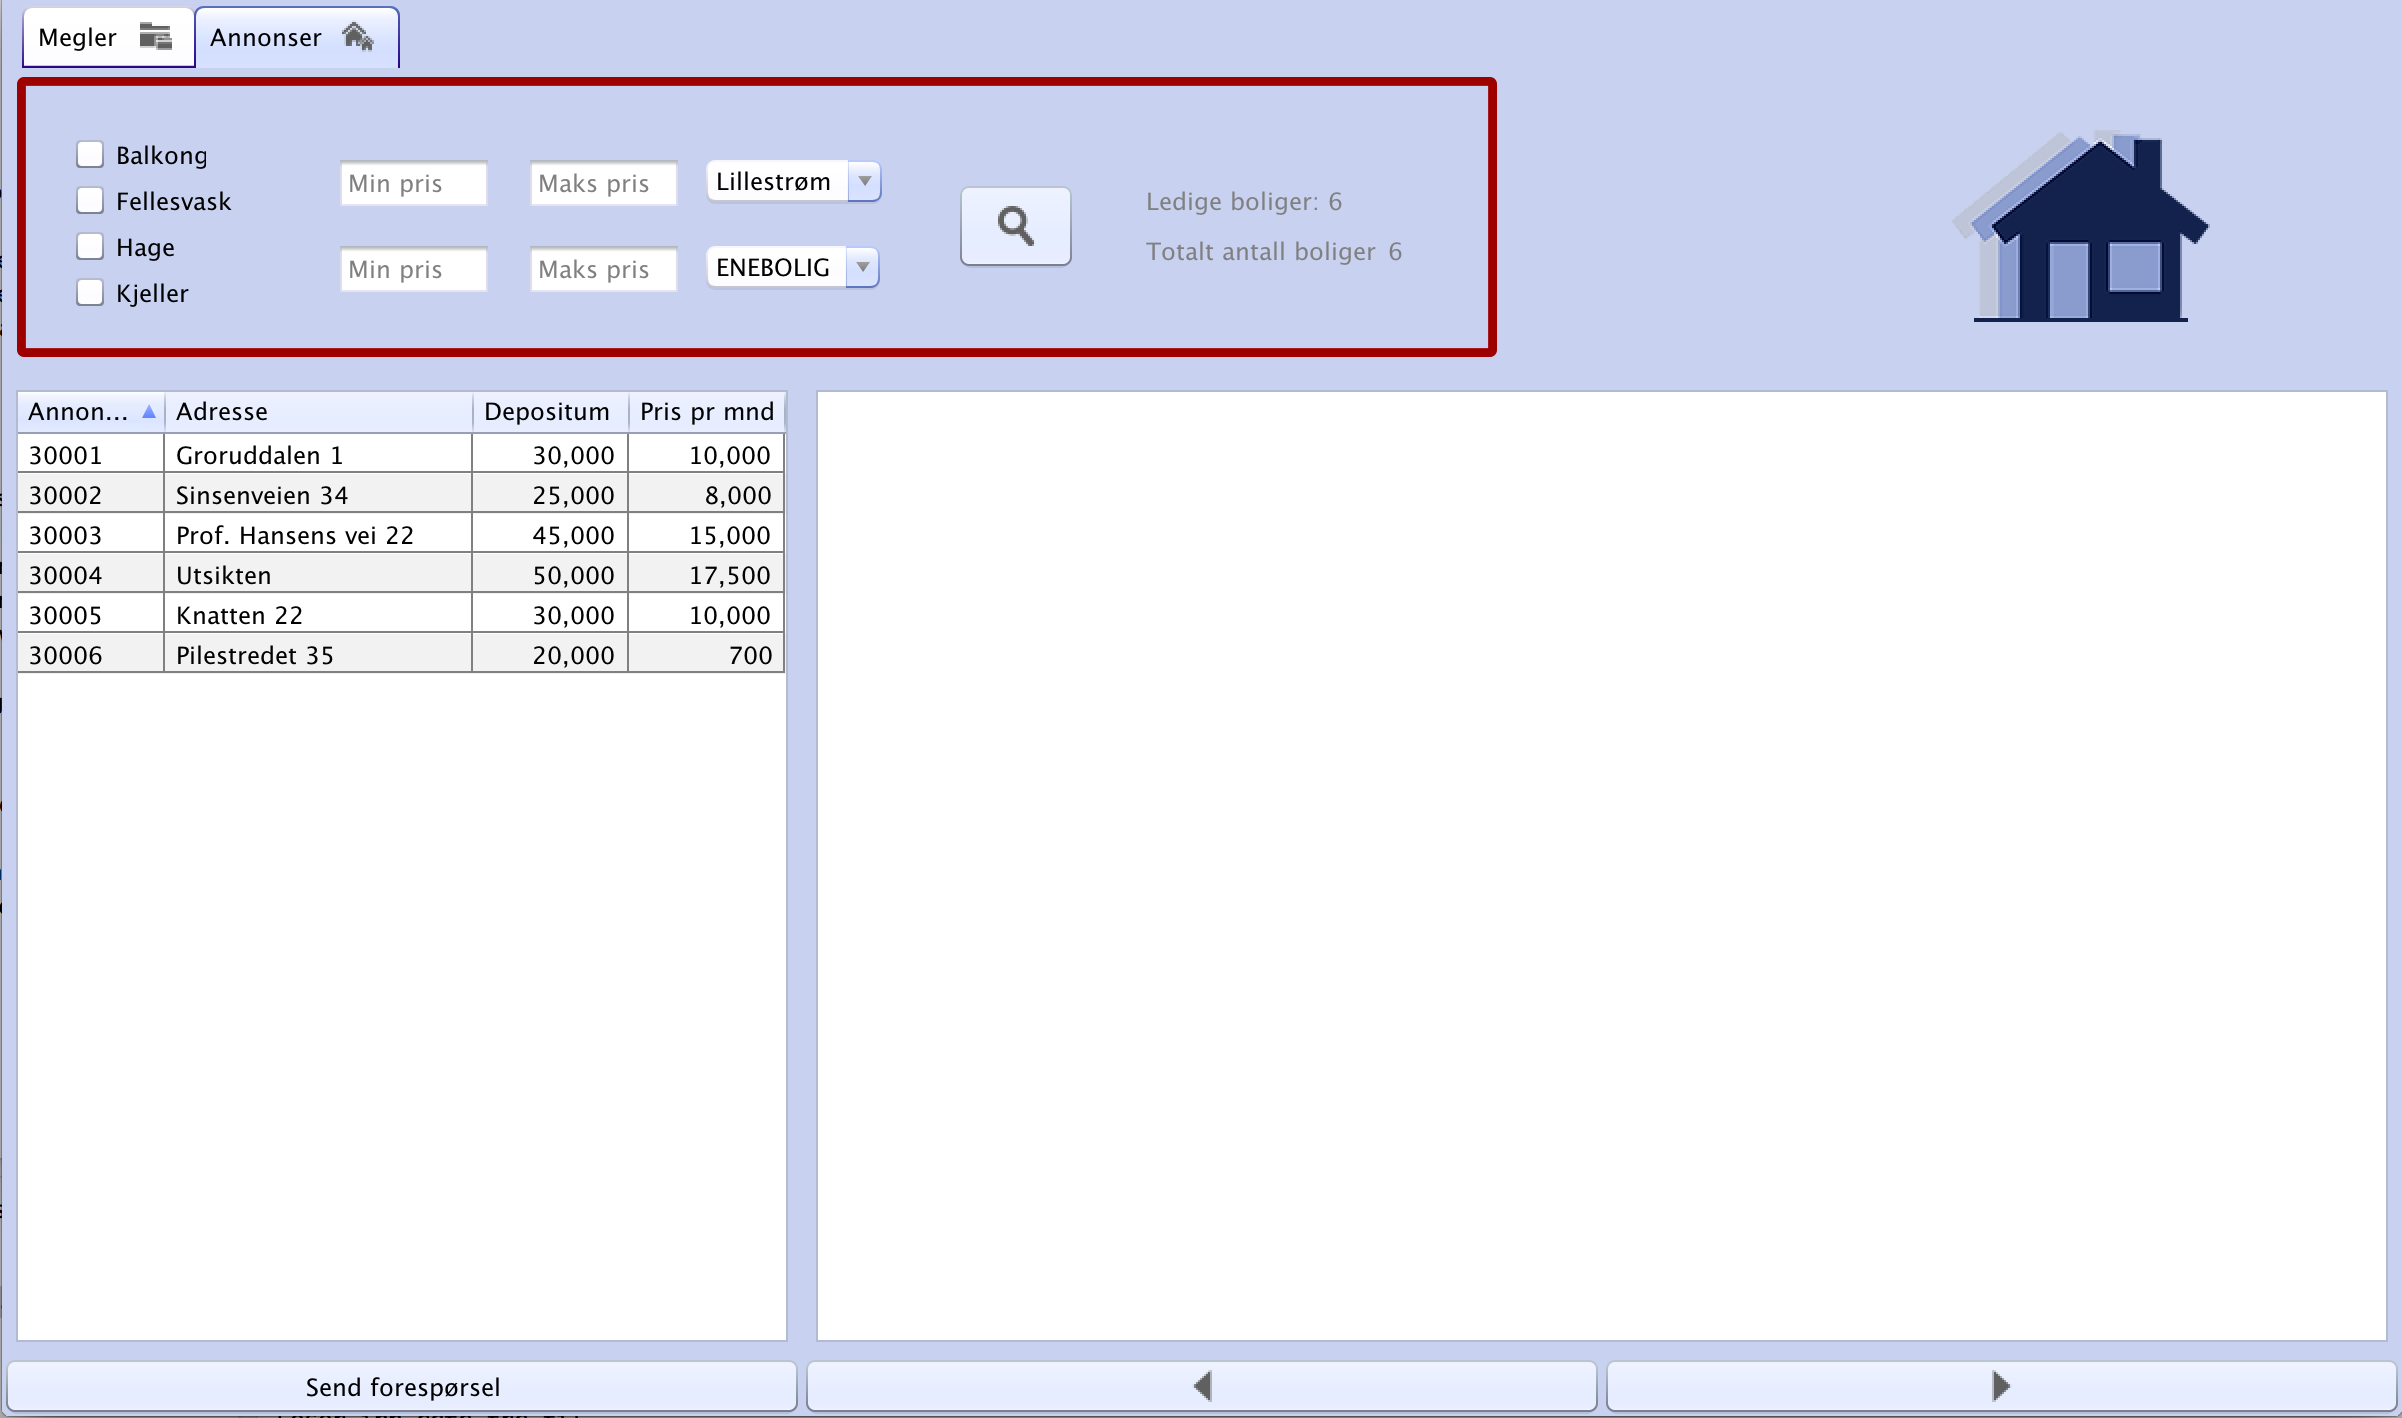
\includegraphics[width=\textwidth,height=\textheight,keepaspectratio]{./img/brukerveiledning/2.png}
 \caption{Filterpanel.}
 \label{fig:bv:2}
\end{figure}




\newpage
\subsection{Resultattabell}
Dette er venstre del av programvinduet, markert i rødt på figur \ref{fig:bv:3}.
Her vil resultater av et evnt. utført søk vises.

En har mulighet til å sortere på annonse ID, Adresse, Depositum, og pris per mnd øverst i
resultatvinduet. Du kan bla igjennom annonser ved å bruke pil opp, eller pil ned knappene, eller
alternativt bruke “fram og tilbake” knappene nederst til høyre i programvinduet.


\begin{figure}[h!]
 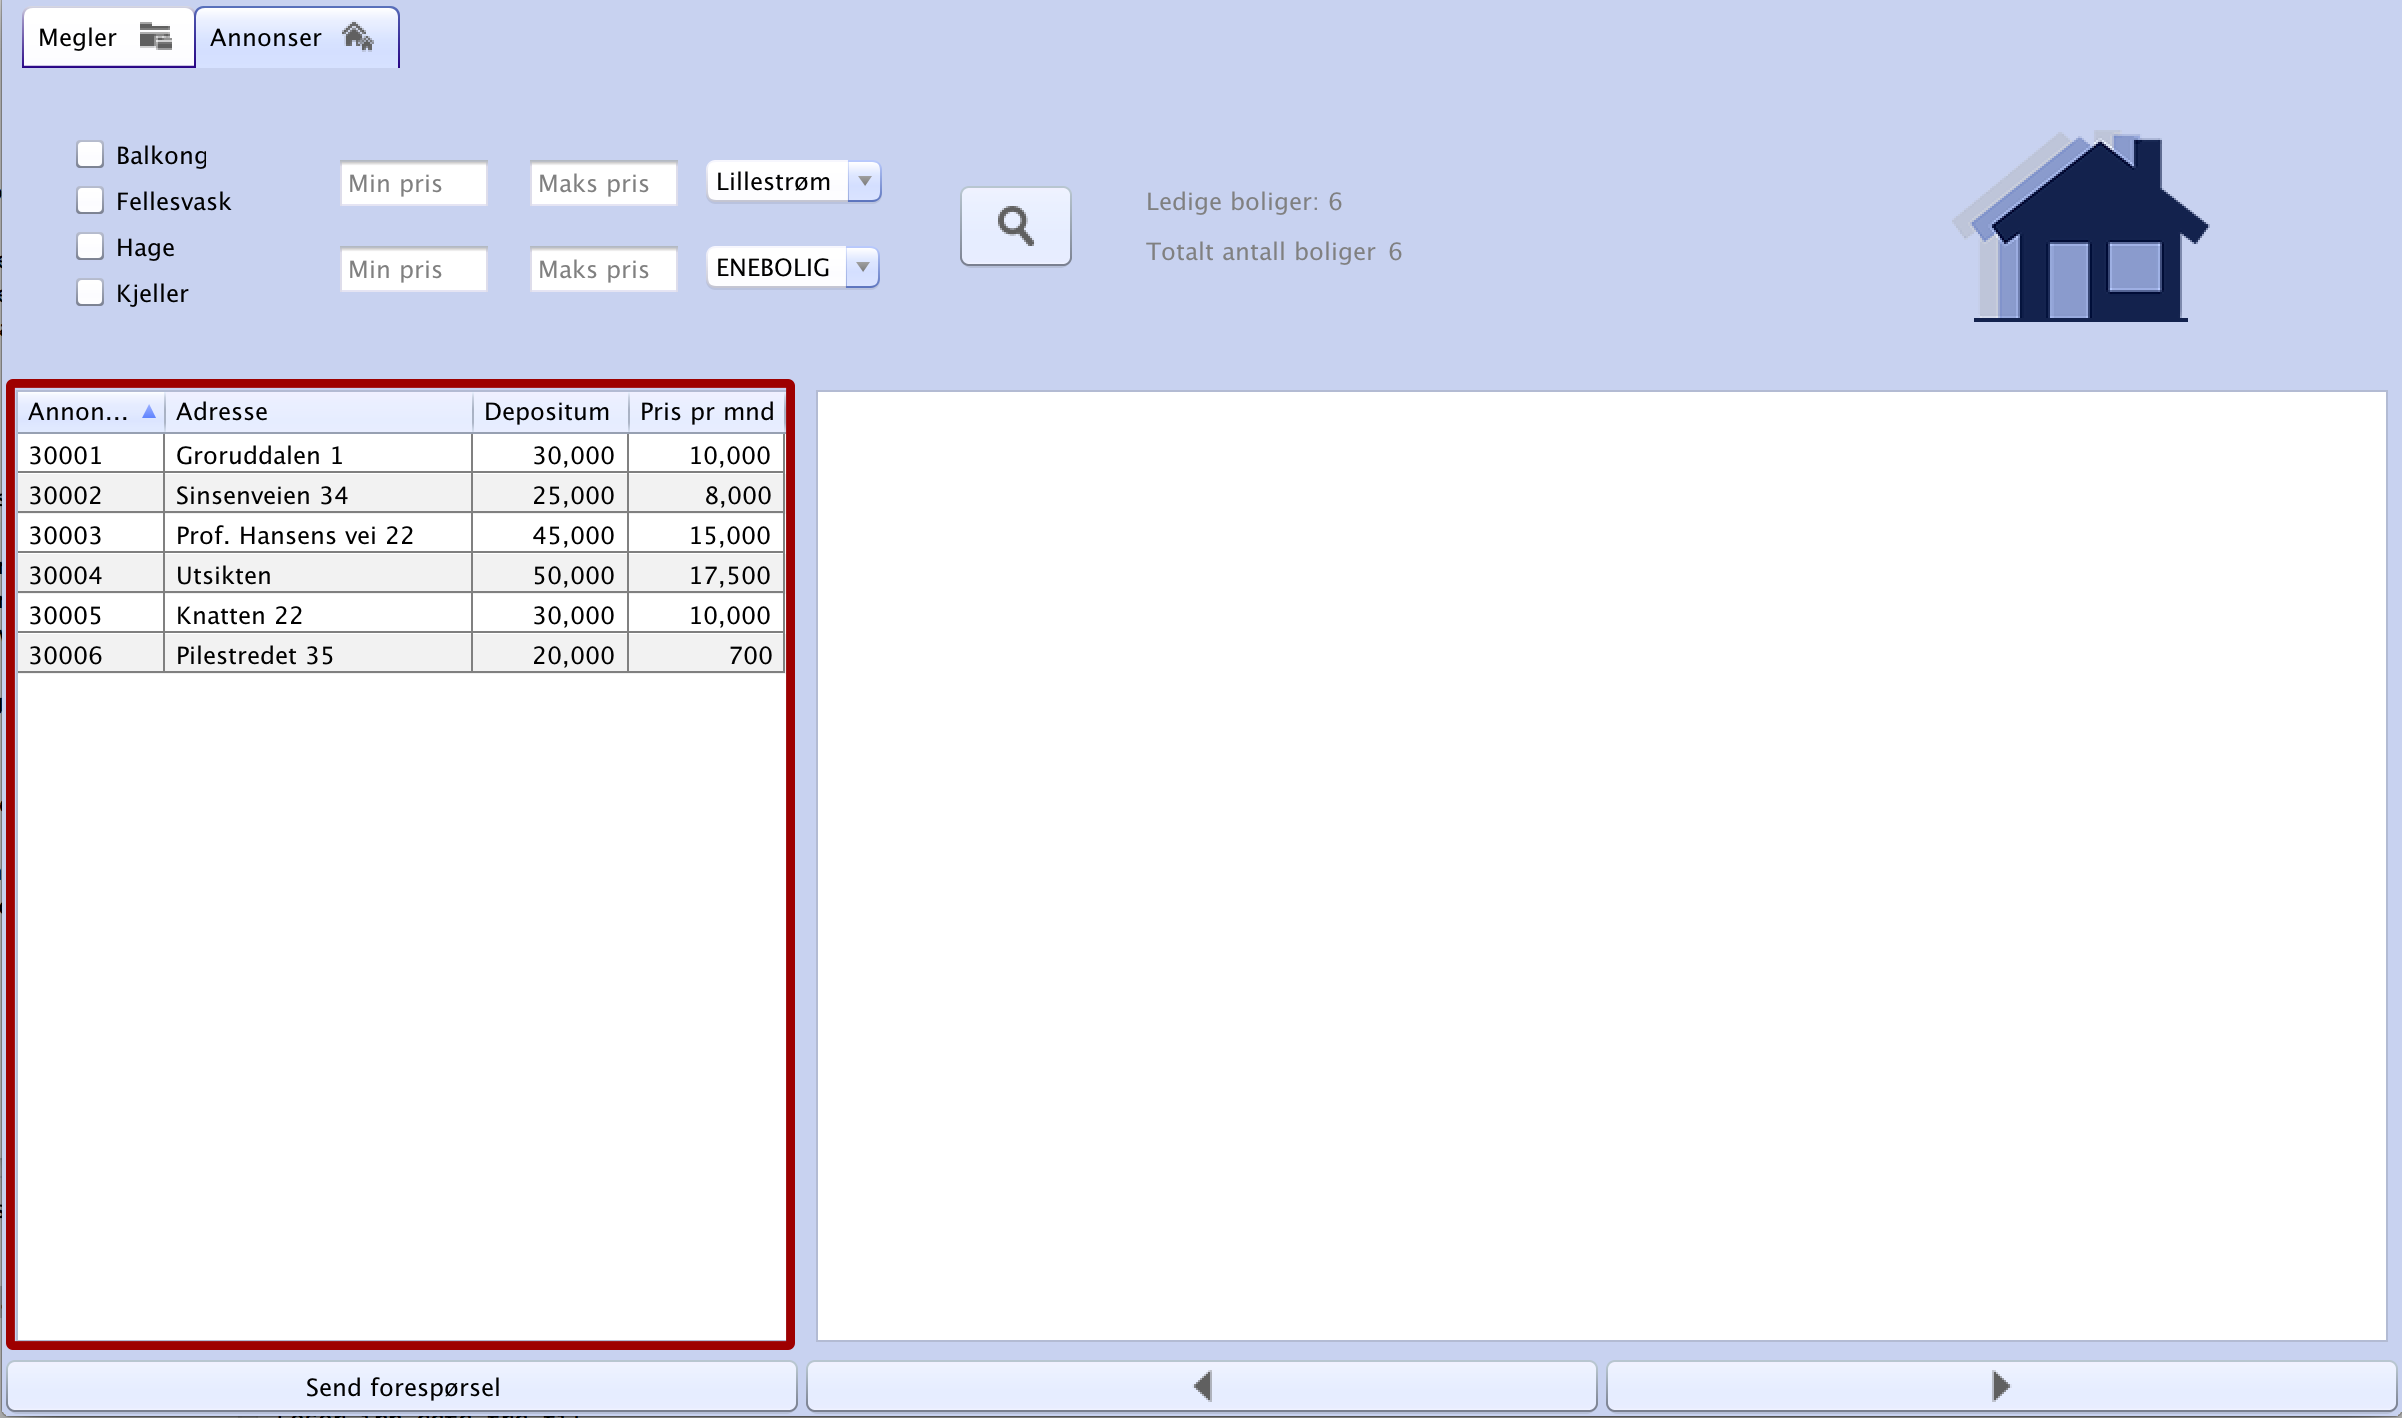
\includegraphics[width=\textwidth,height=\textheight,keepaspectratio]{./img/brukerveiledning/3.png}
 \caption{Resultattabell.}
 \label{fig:bv:3}
\end{figure}

Trykk på et treff i tabellen for å få fram flere detaljer om den valgte boligen i...




\newpage
\subsection{Visningspanel}

Her vil detaljer rundt valgt bolig (i resultattabellen) vises, markert i rødt på figur \ref{fig:bv:4}.


\begin{figure}[h!]
 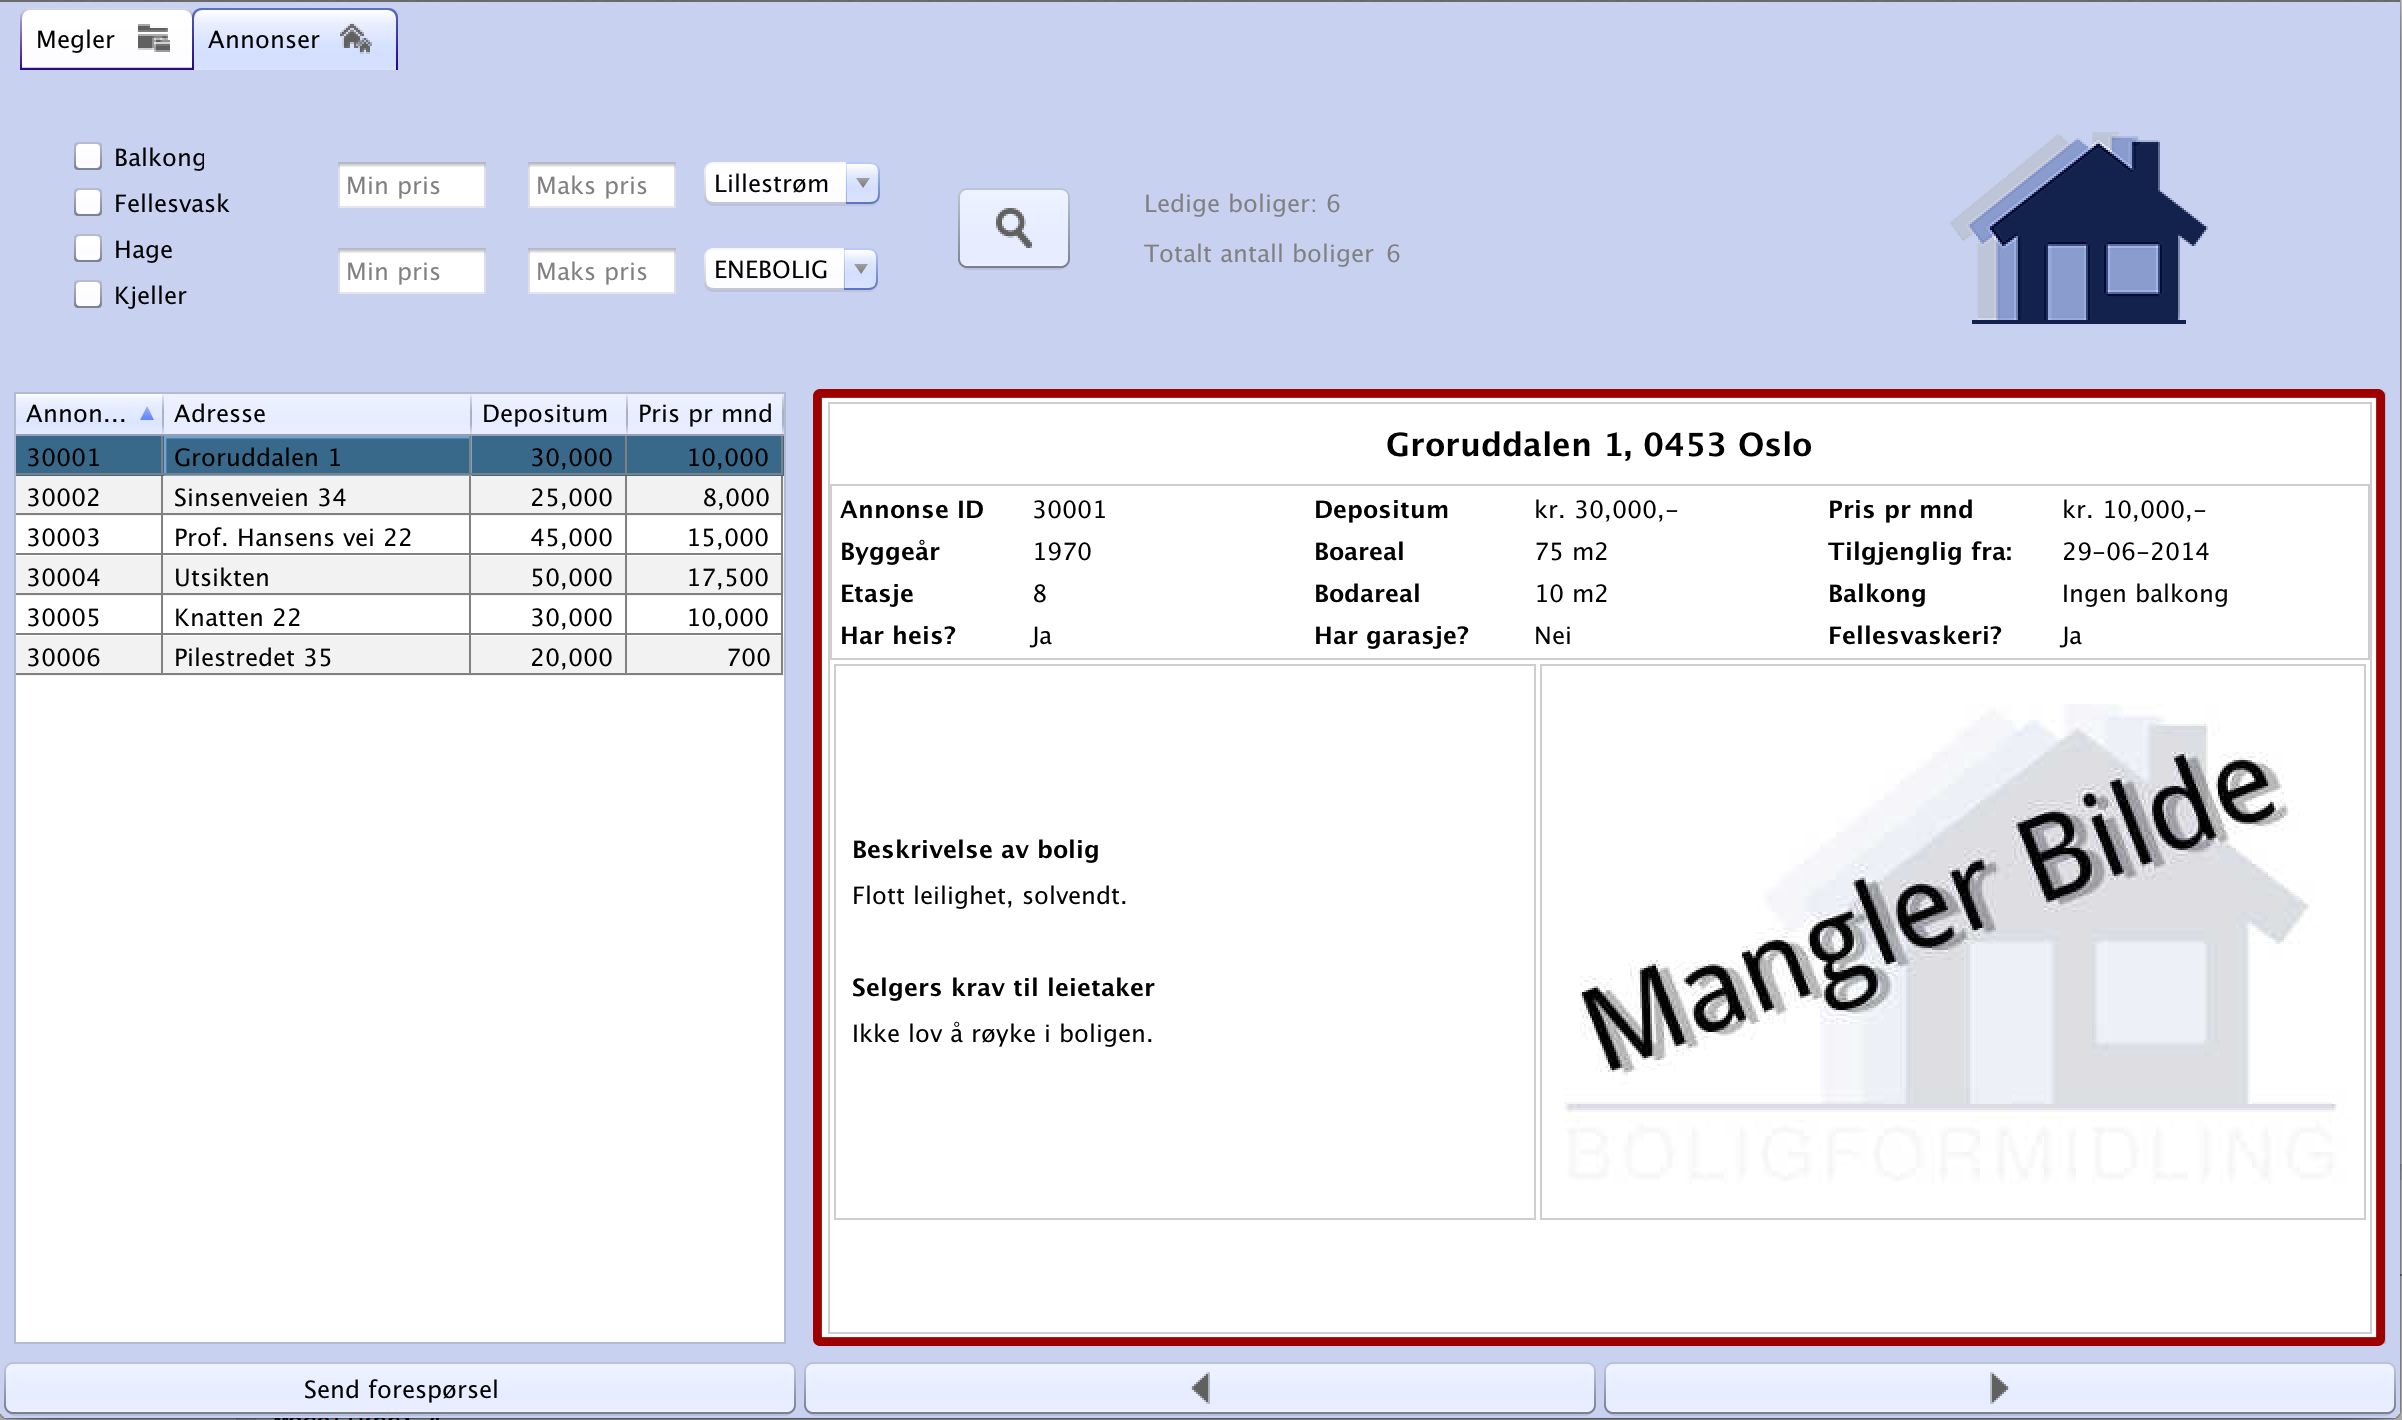
\includegraphics[width=\textwidth,height=\textheight,keepaspectratio]{./img/brukerveiledning/4.png}
 \caption{Visningspanel.}
 \label{fig:bv:4}
\end{figure}






\subsection{Forespørsel/søknad}
Trykk på “Send forespørsel” knappen nede i venstre hjørne av programmet (alternativt CTRL-F),
for sende inn din søknad på valgt bolig. Du vil da bli spurt om å akseptere evnt. spesielle vilkår
(figur \ref{fig:bv:5}) for den valgte boligen.

\begin{figure}[h!]
\center
 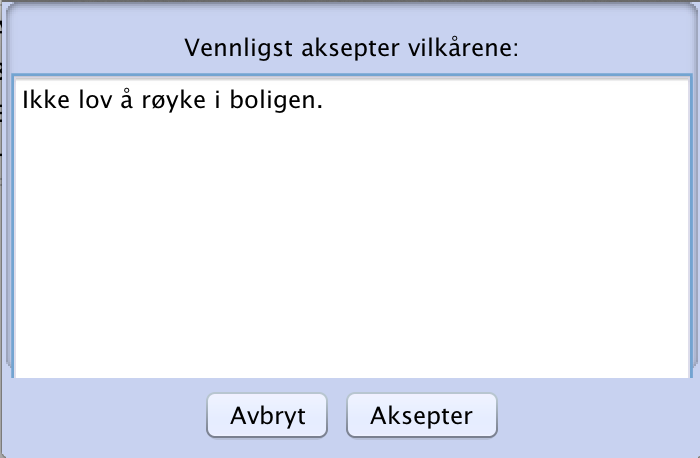
\includegraphics[scale=0.7]{./img/brukerveiledning/5.png}
 \caption{Forespørsel og krav fra utleier.}
 \label{fig:bv:5}
\end{figure}


Etter å evnt. ha akseptert vilkårene for den aktuelle boligen, så får en opp et nytt vindu med
mulighet for å skrive inn personalia mm. og sende inn søknad på boligen, som vist på figur \ref{fig:bv:6}.


\begin{figure}[h!]
\center
 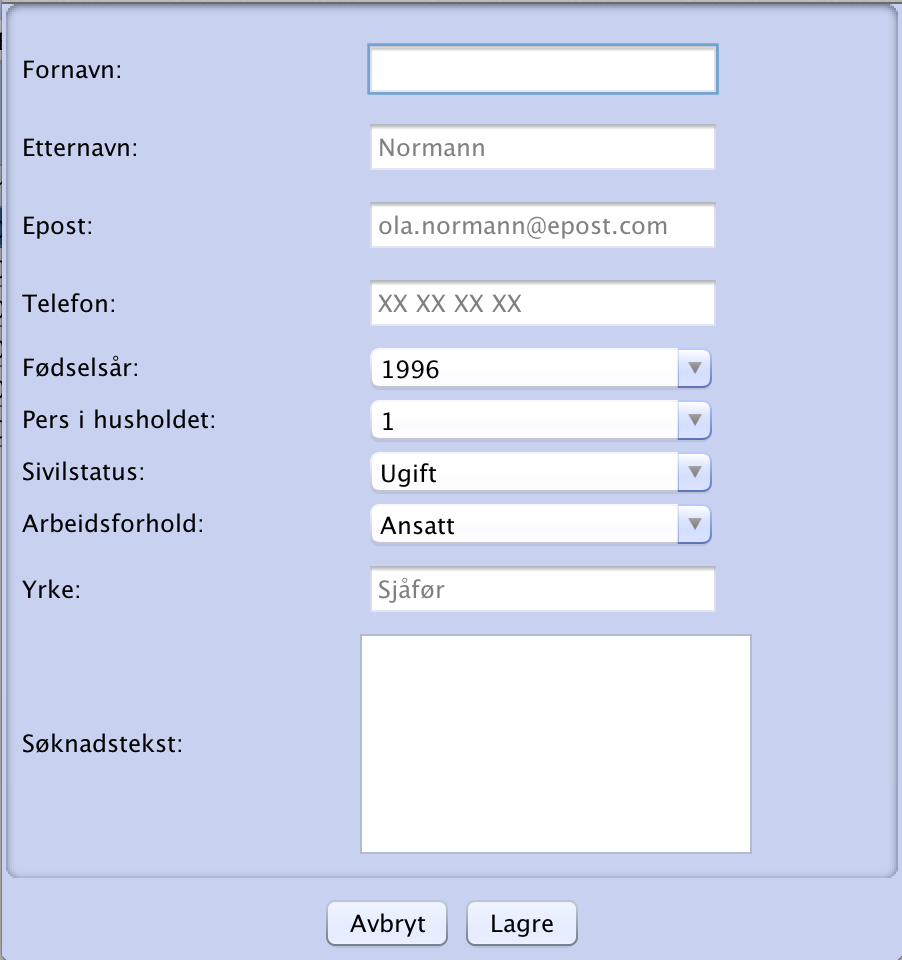
\includegraphics[scale=0.7]{./img/brukerveiledning/6.png}
 \caption{Registrering for leietaker.}
 \label{fig:bv:6}
\end{figure}





%////////////////////////////////////////////
\newpage
\section{Megler/administrasjon}

\subsection{Pålogging}

Ved å velge “Megler”-arkfanen, så vil du først bli spurt om å logge deg inn som vist på figur \ref{fig:bv:7}.
Tast inn ditt brukernavn og passord, og trykk “Enter” for å logge inn, eller evnt. ved å trykke på “Ok”
knappen. Velger du “Avbryt” vil du komme tilbake til Annonse-arkfanen igjen.

\begin{figure}[h!]
\center
 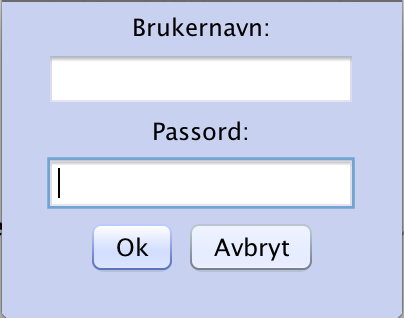
\includegraphics[scale=0.7]{./img/brukerveiledning/7.png}
 \caption{Pålogging for megler.}
 \label{fig:bv:7}
\end{figure}




\newpage
\subsection{Menyer}
I den øverste delen av programmet som vist på figur \ref{fig:bv:8}, så har du en knappegruppe som er ansvarlig
for administrasjon, mer spesifikt funksjonalitet for å opprette ny utleier, ny bolig, ny annonse, og
 ny kontrakt.

Hvilke av disse funksjonene / knappene som er mulig å bruke, er avhengig av hvilken type
objekt du har valgt i i vinduet for søkeresultater. Mer spesifikt:

\begin{description}
\item[Ny Utleier] -
Kan brukes når som helst. \texttt{CTRL-U}
\item[Ny Bolig] -
Kan brukes etter å ha søkt og valgt blant utleiere. \texttt{CTRL-B}
\item[Ny Annonse] -
Kan brukes etter å ha søkt og valgt blant boliger. \texttt{CTRL-A}
\item[Ny Kontrakt] -
Kan brukes etter å ha søkt og valgt blant søknader. \texttt{CTRL-K}
\end{description}





\subsection{Søkepanel}
I øverste delen av programmet som vist på figur \ref{fig:bv:8}, så har du mulighet til å søke blant
boligsøknader, annonser, boliger, utleiere, leietakere, og eksisterende kontrakter.
Du må velge en kategori på venstre siden av søkefeltet for å kunne ta i bruk søkefunksjonaliteten,
ved hjelp av å trykke “Enter”, eller ved å enkelt og greit trykke på “søkeknappen”.


\begin{figure}[h!]
 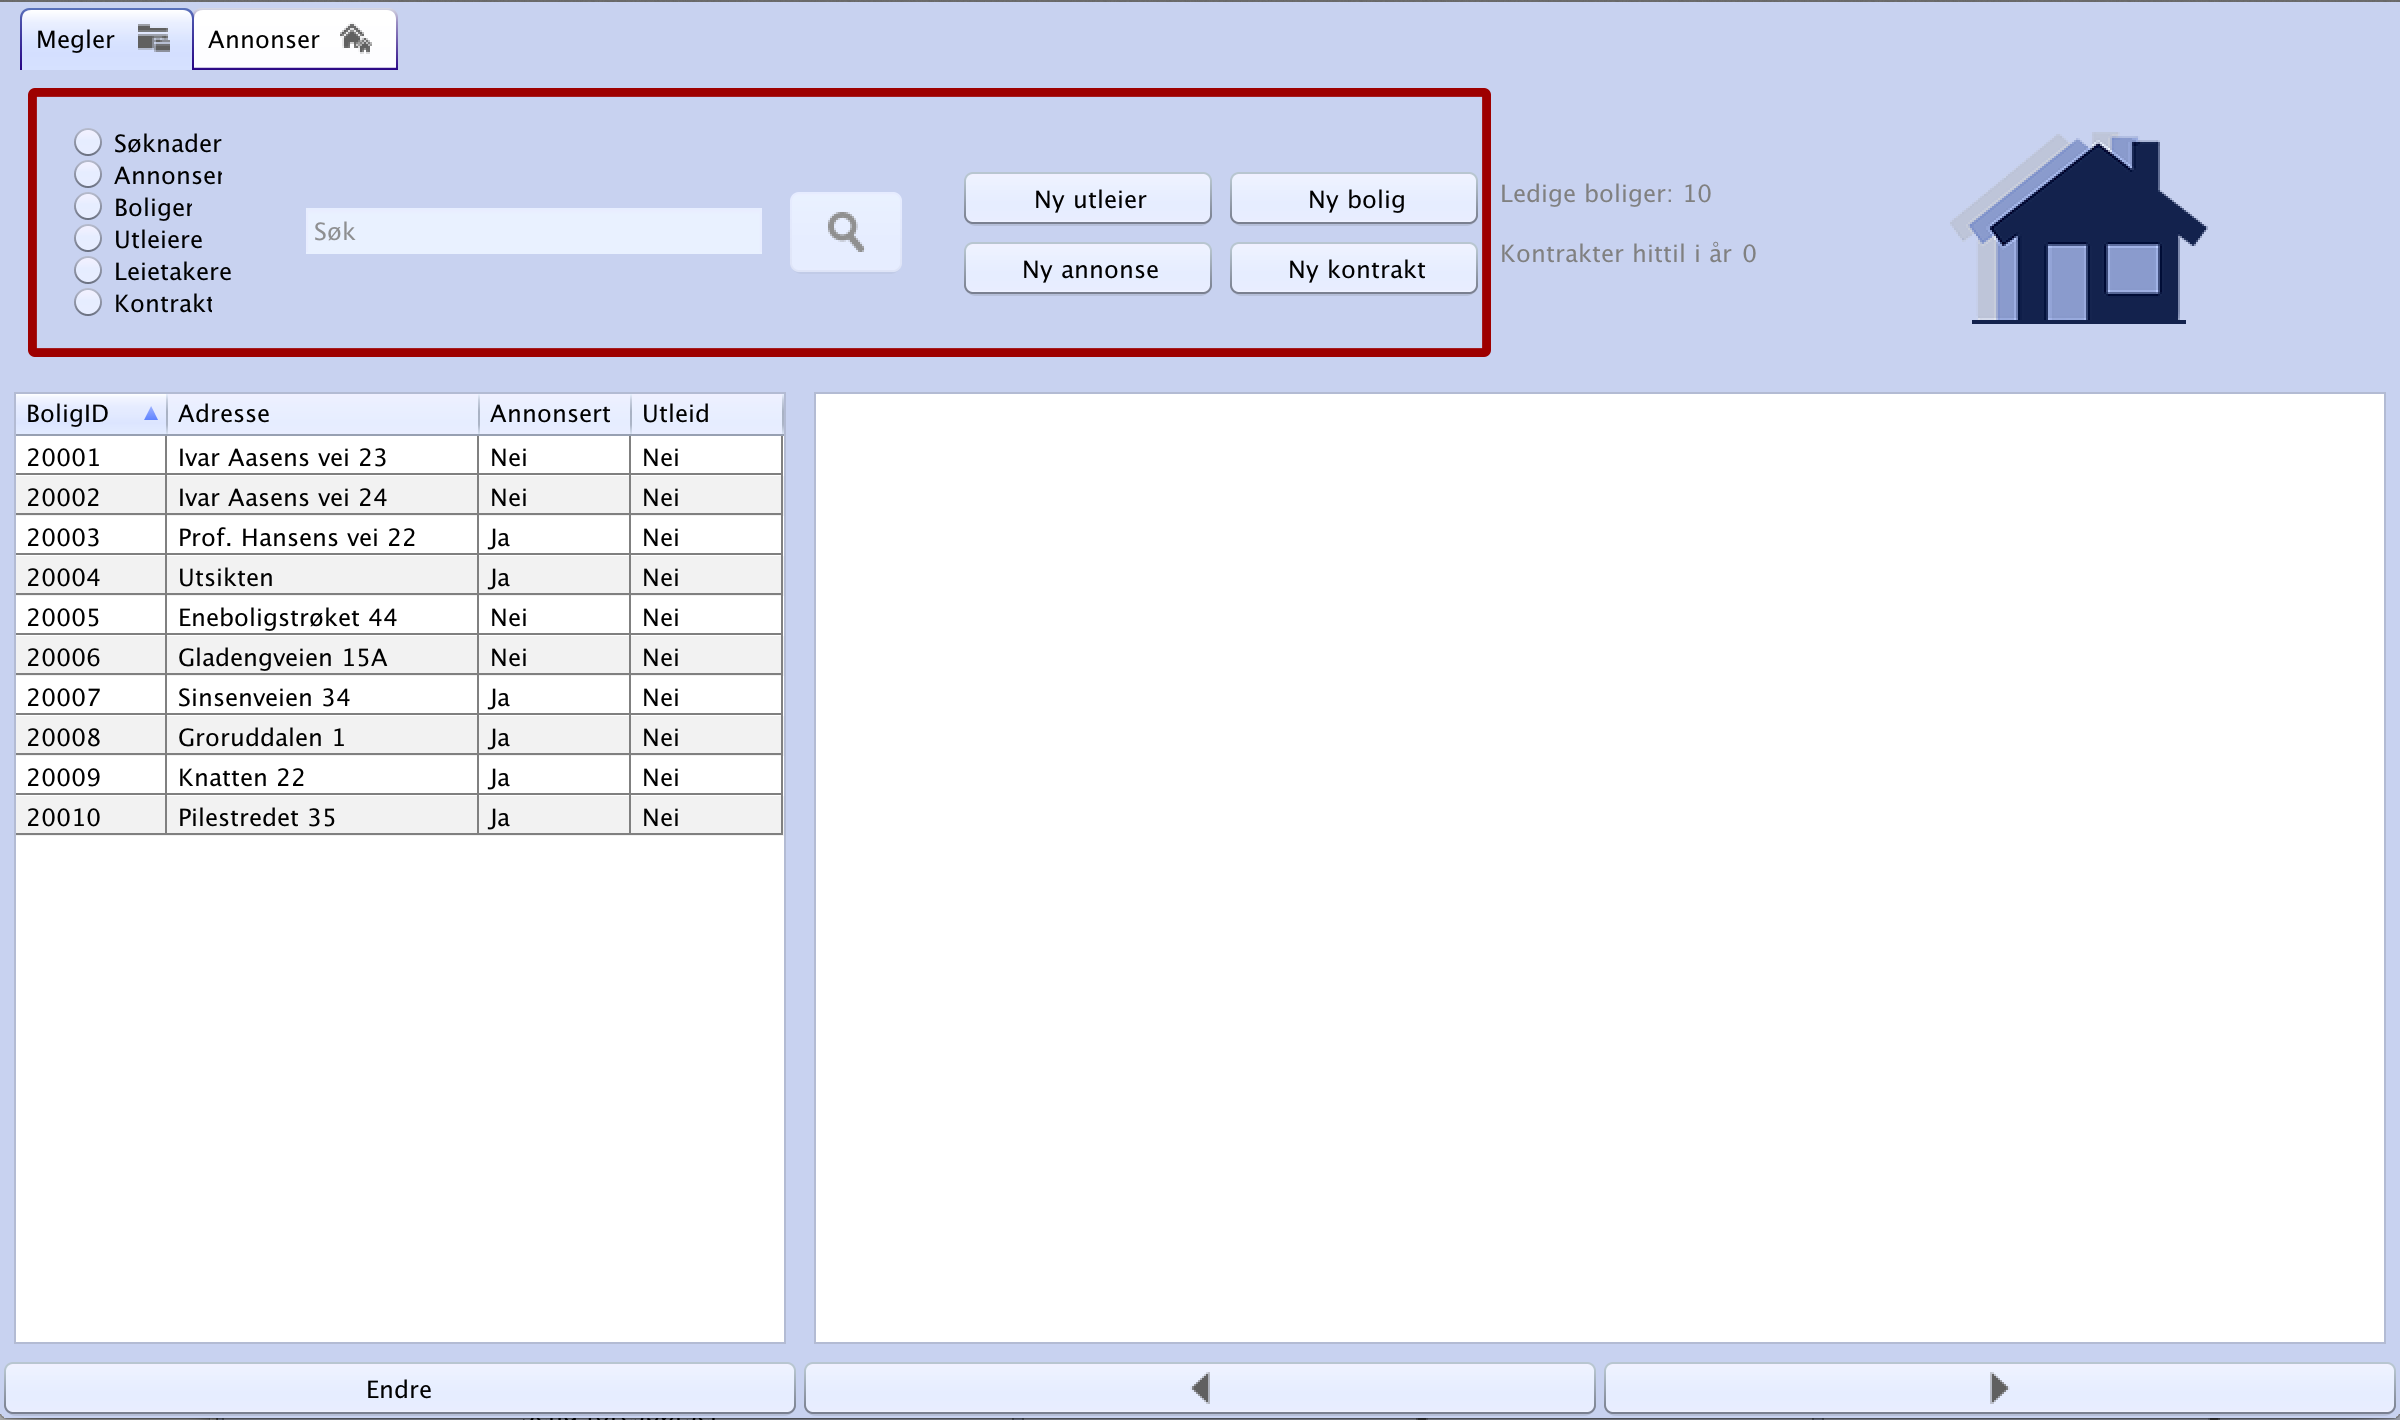
\includegraphics[width=\textwidth,height=\textheight,keepaspectratio]{./img/brukerveiledning/8.png}
 \caption{Søkepanel.}
 \label{fig:bv:8}
\end{figure}


\newpage
\subsection{Resultattabell}

Dette er venstre del av programvinduet, markert i rødt på figur \ref{fig:bv:9}. 
Her vil resultater av et evnt. utført søk vises. 

En har mulighet til å sortere på diverse kriterier øverst i resultatvinduet. Du kan bla igjennom
annonser ved å bruke pil opp, eller pil ned knappene, eller alternativt bruke “fram og tilbake”
knappene nederst til høyre i programvinduet.

\begin{figure}[h!]
 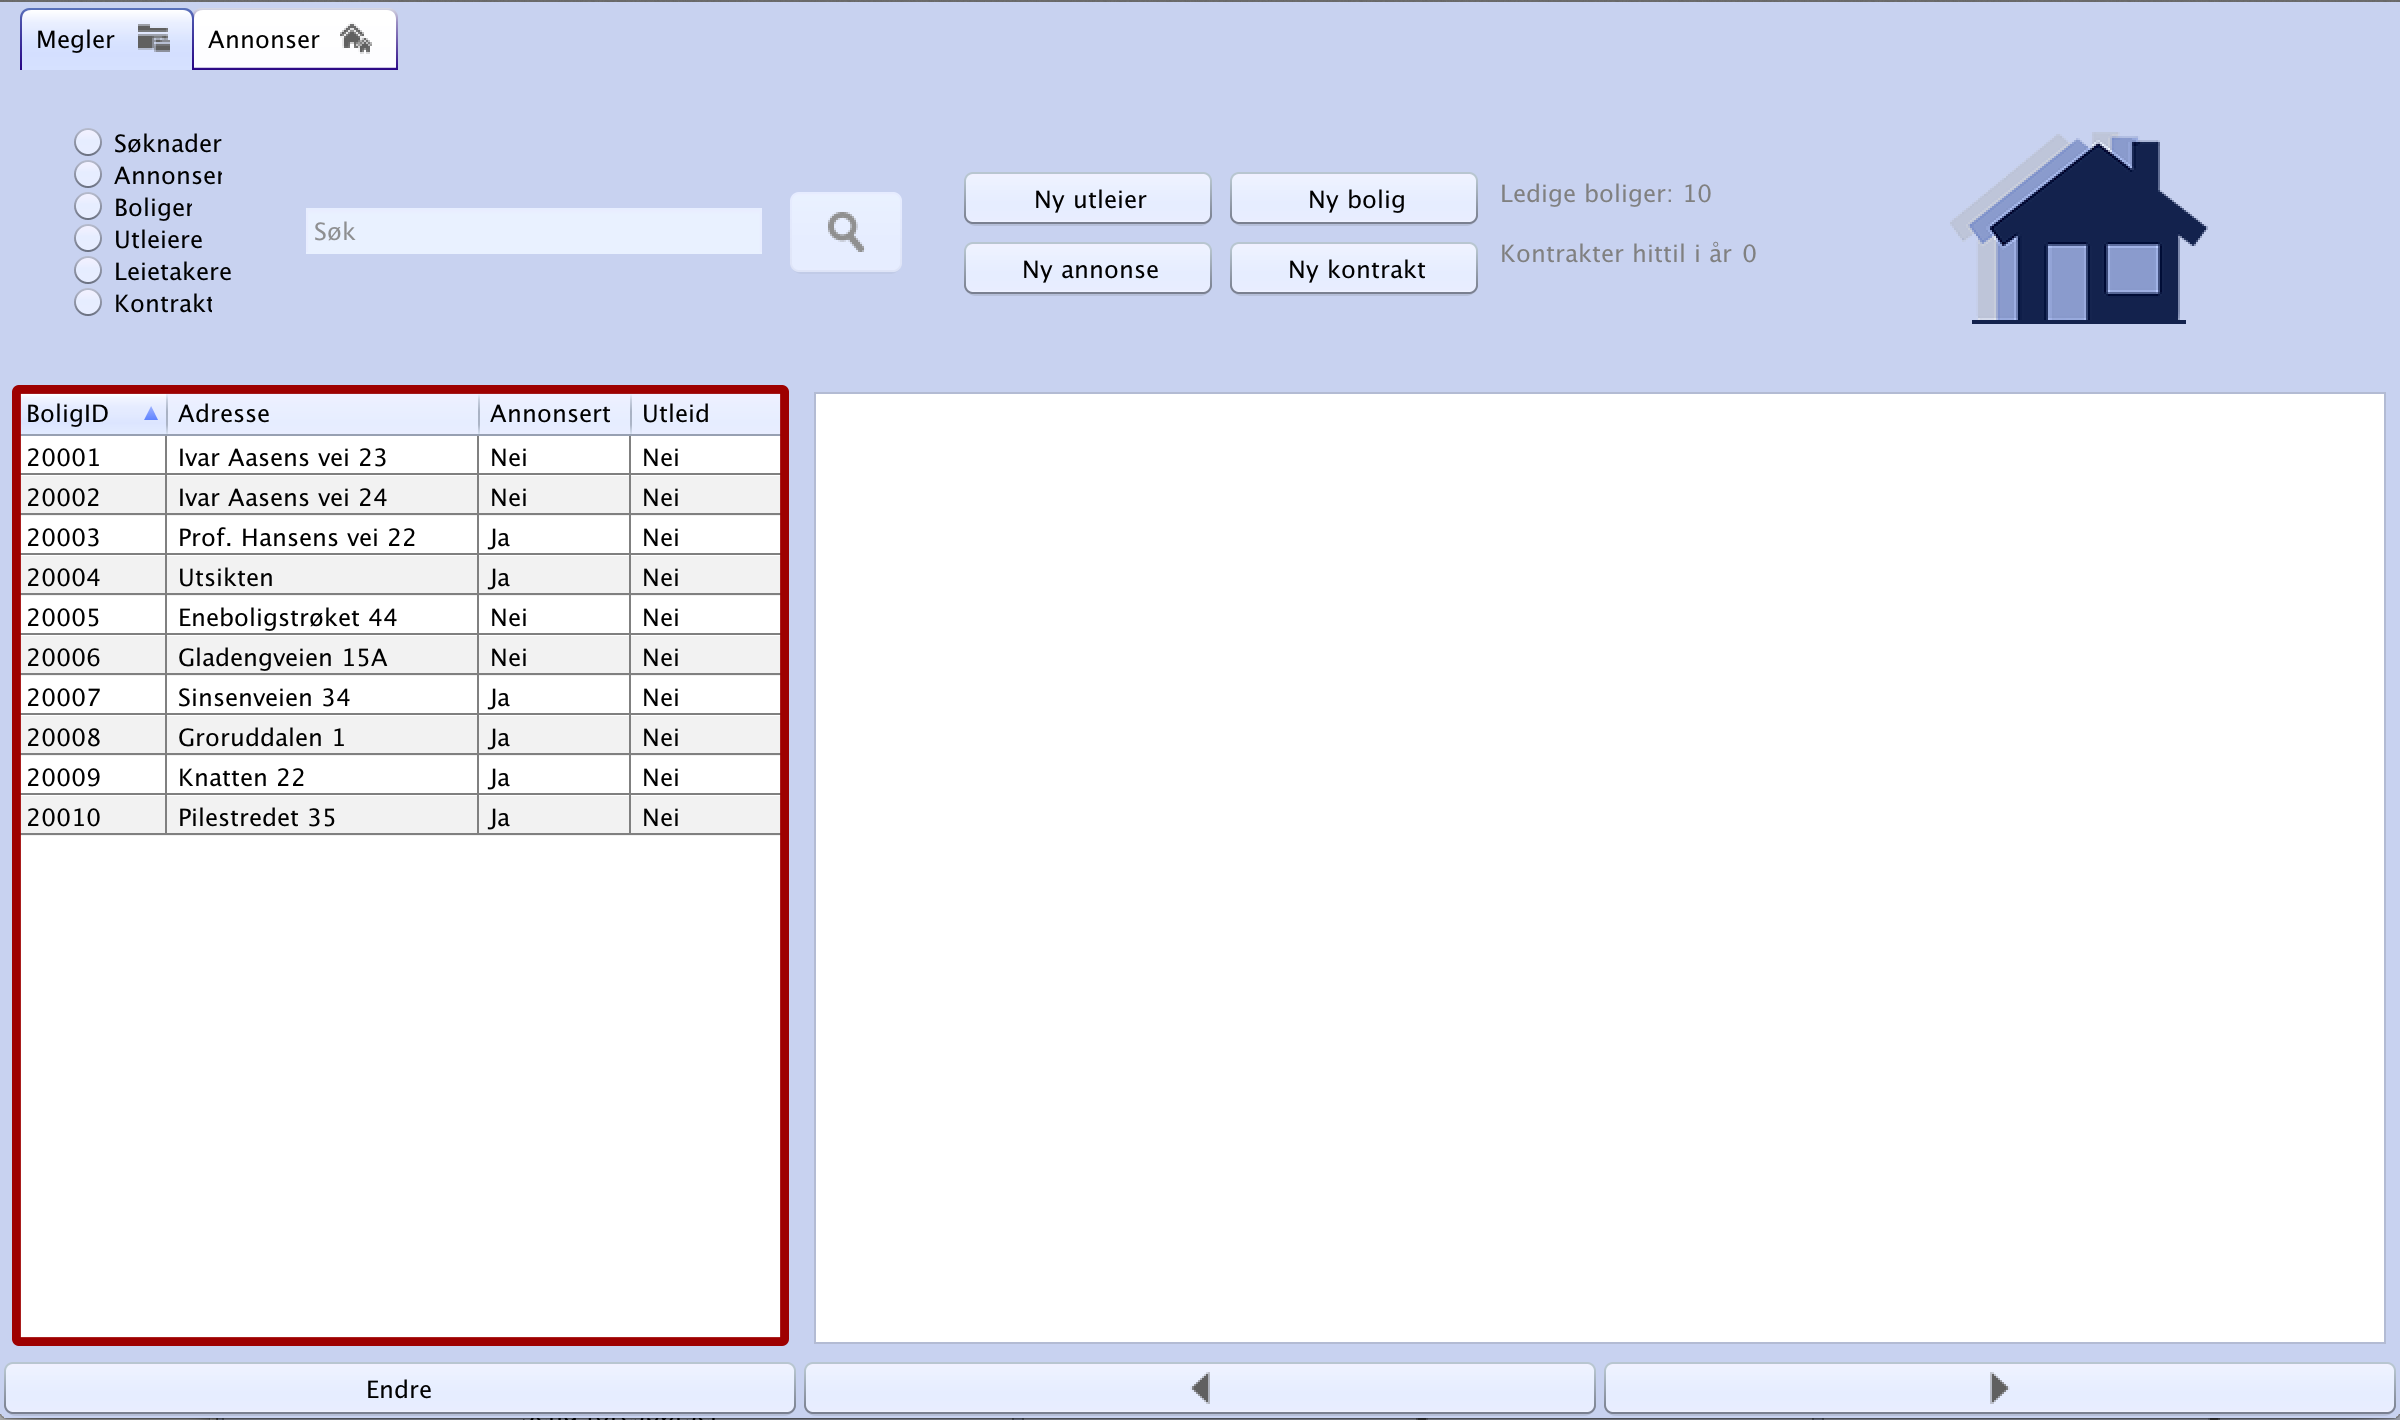
\includegraphics[width=\textwidth,height=\textheight,keepaspectratio]{./img/brukerveiledning/9.png}
 \caption{Resultattabell.}
 \label{fig:bv:9}
\end{figure}


\newpage
\subsection{Visningspanel}

Her vil detaljer rundt valgt objekt (i resultattabellen) vises, markert i rødt på figur \ref{fig:bv:10}.


\begin{figure}[h!]
 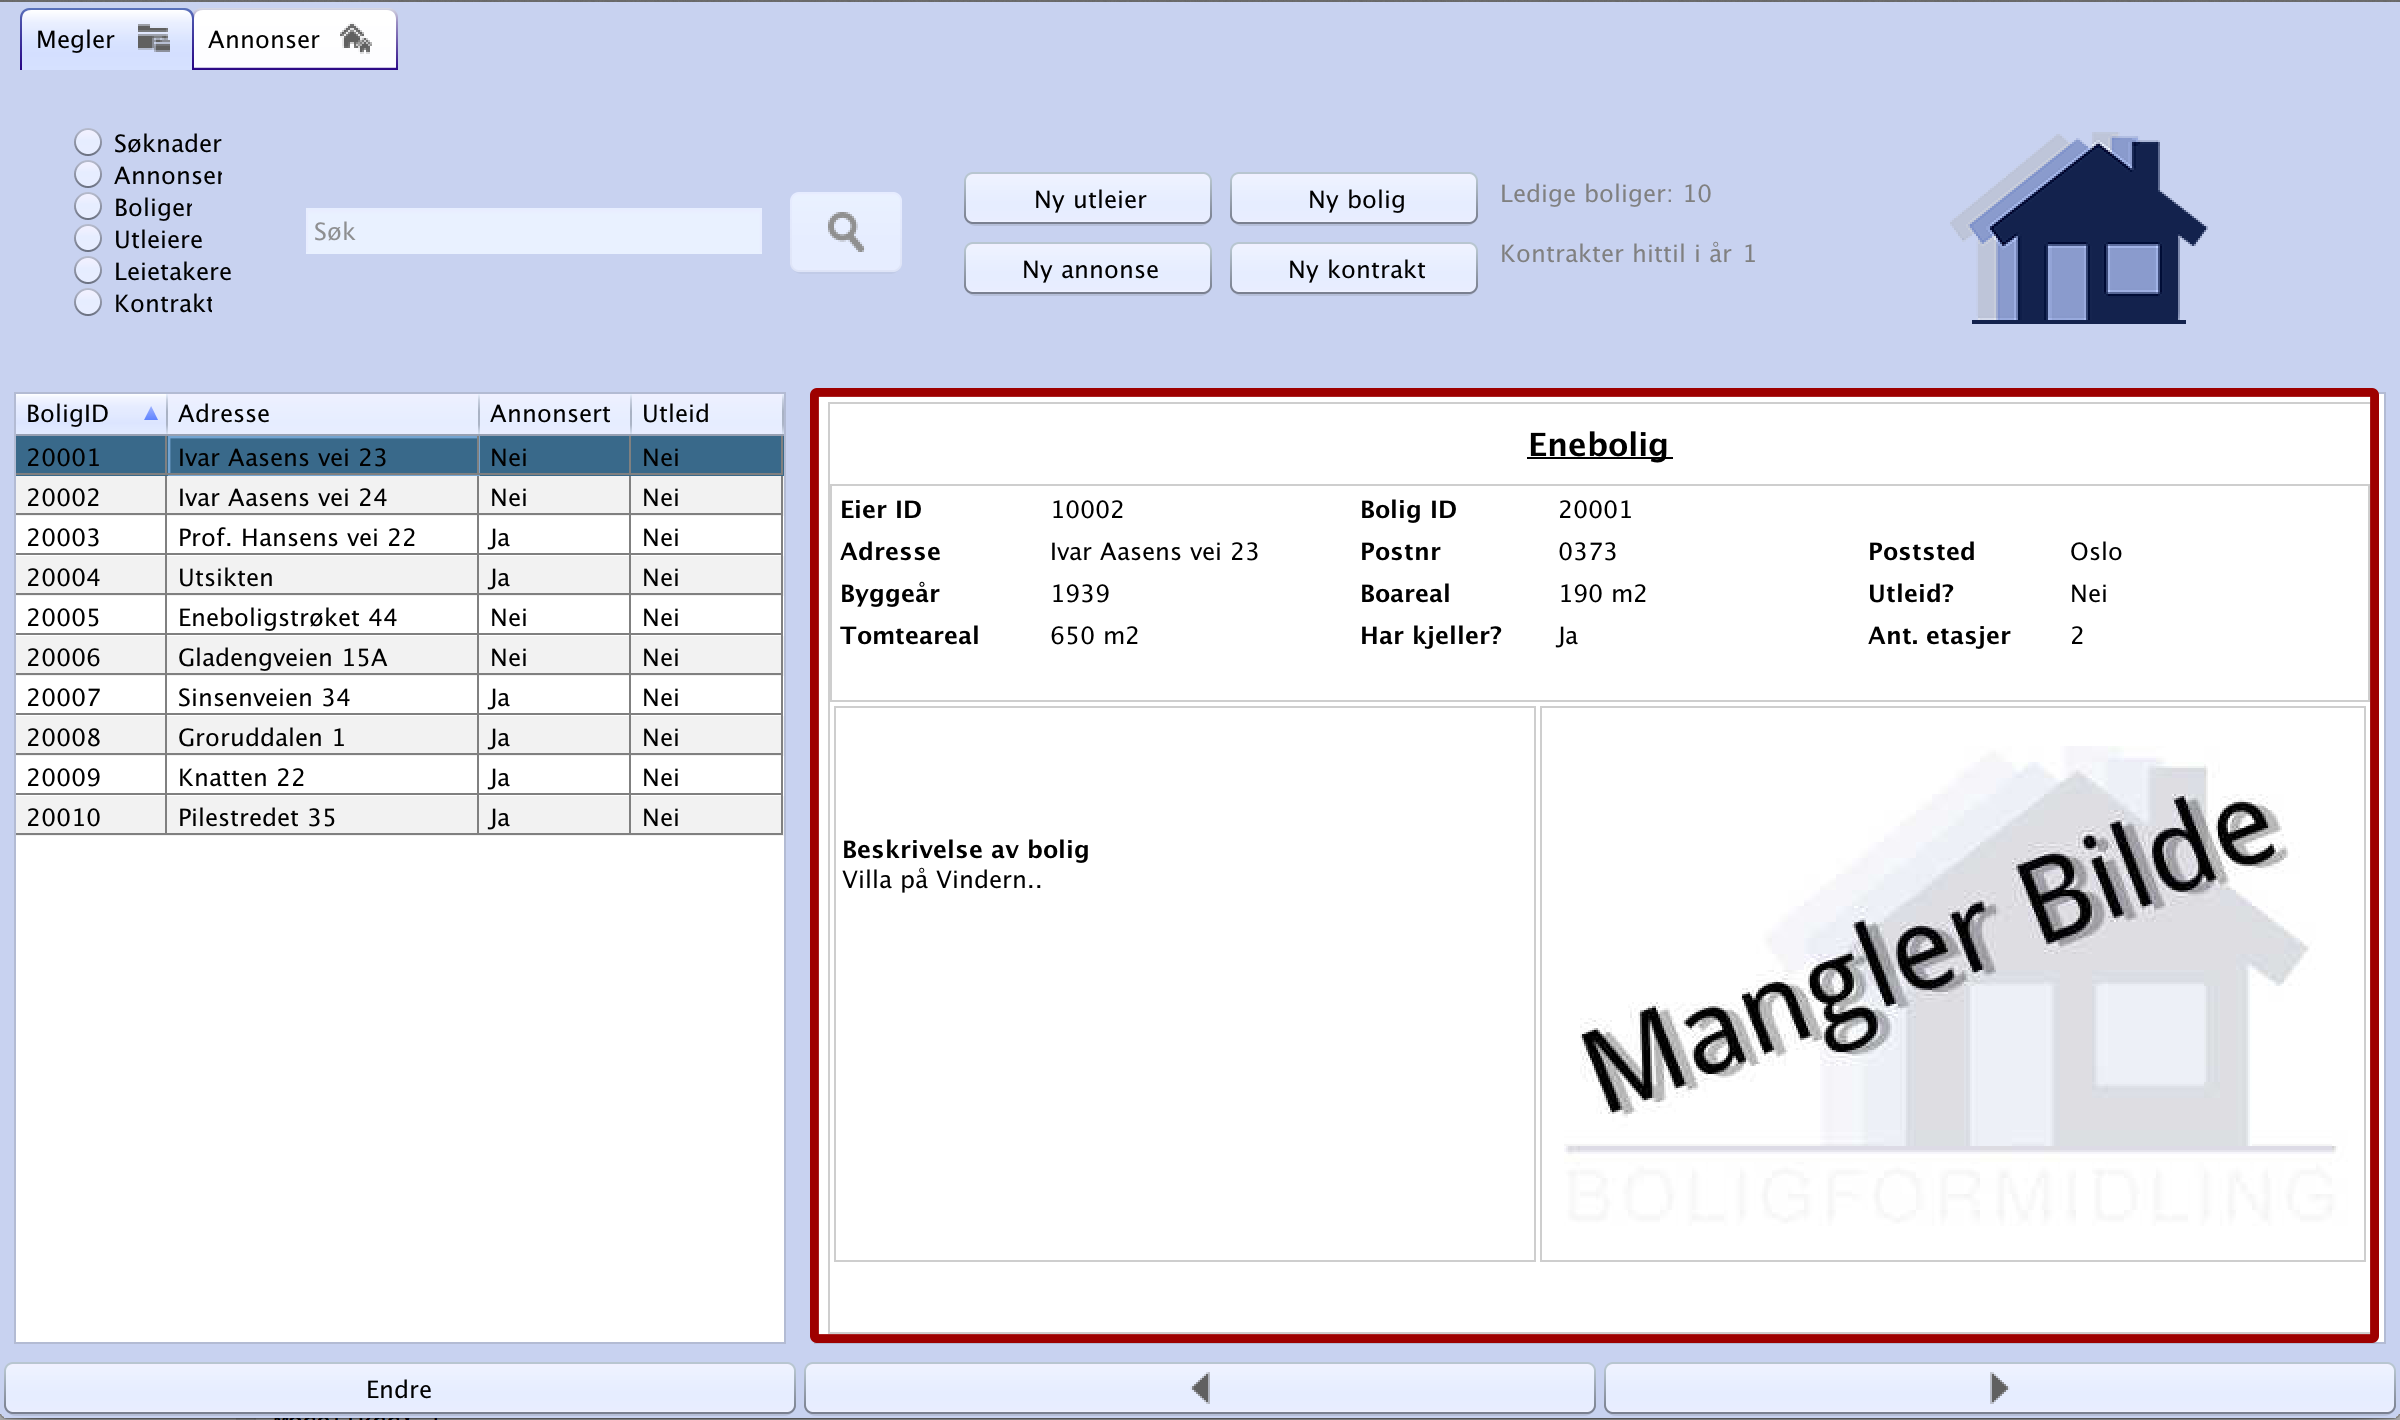
\includegraphics[width=\textwidth,height=\textheight,keepaspectratio]{./img/brukerveiledning/10.png}
 \caption{Visningspanel.}
 \label{fig:bv:10}
\end{figure}



\newpage
\subsection{Utleieradministrasjon}

Ved å søke blant utleiere, velge en person i listen, og trykke på “Endre” knappen nedest i venstre
hjørne av programvinduet, så har en mulighet til å gjøre endringer i informasjon lagret om
vedkommende, som vist på figur \ref{fig:bv:11}.

\begin{figure}[h!]
\center
 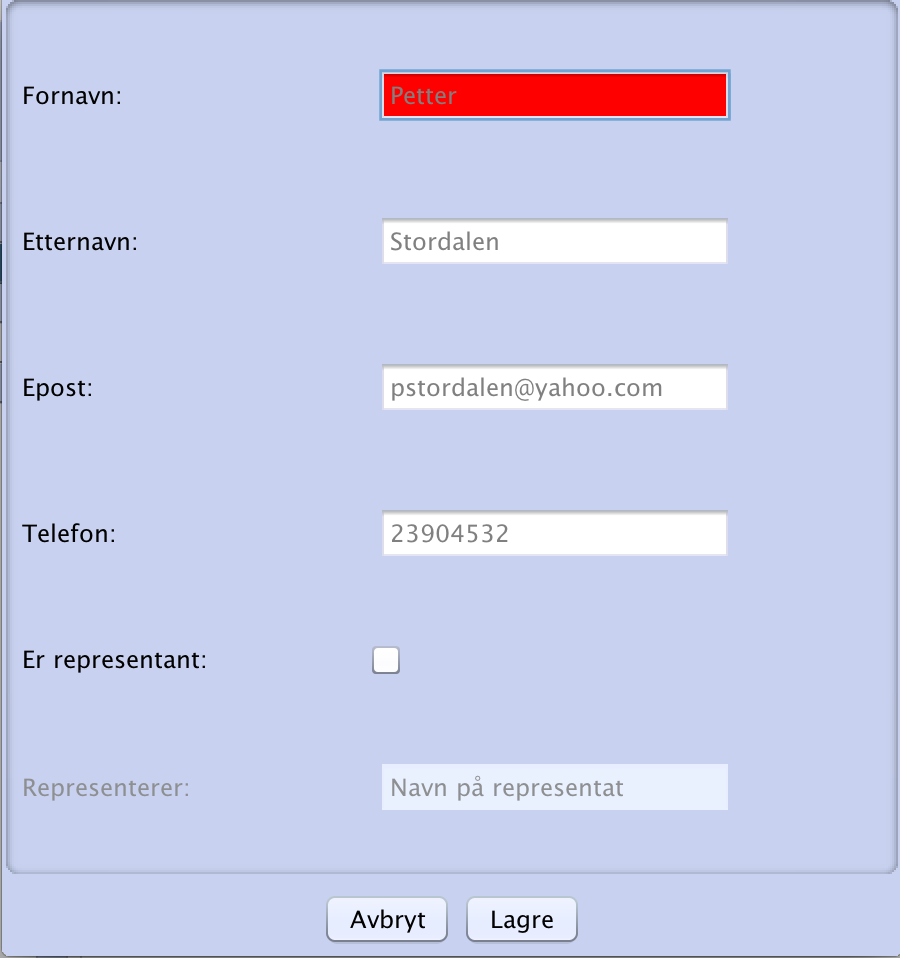
\includegraphics[scale=0.5]{./img/brukerveiledning/11.png}
 \caption{Utleieradministrasjon.}
 \label{fig:bv:11}
\end{figure}




\newpage
\subsection{Annonseadministrasjon}
Ved å søke blant annonser, velge en annonse i listen, og trykke på “Endre” knappen nedest i venstre hjørne av programvinduet, så har en mulighet til å gjøre endringer i informasjon lagret om annonsen, som vist på figur \ref{fig:bv:12}.

\begin{figure}[h!]
 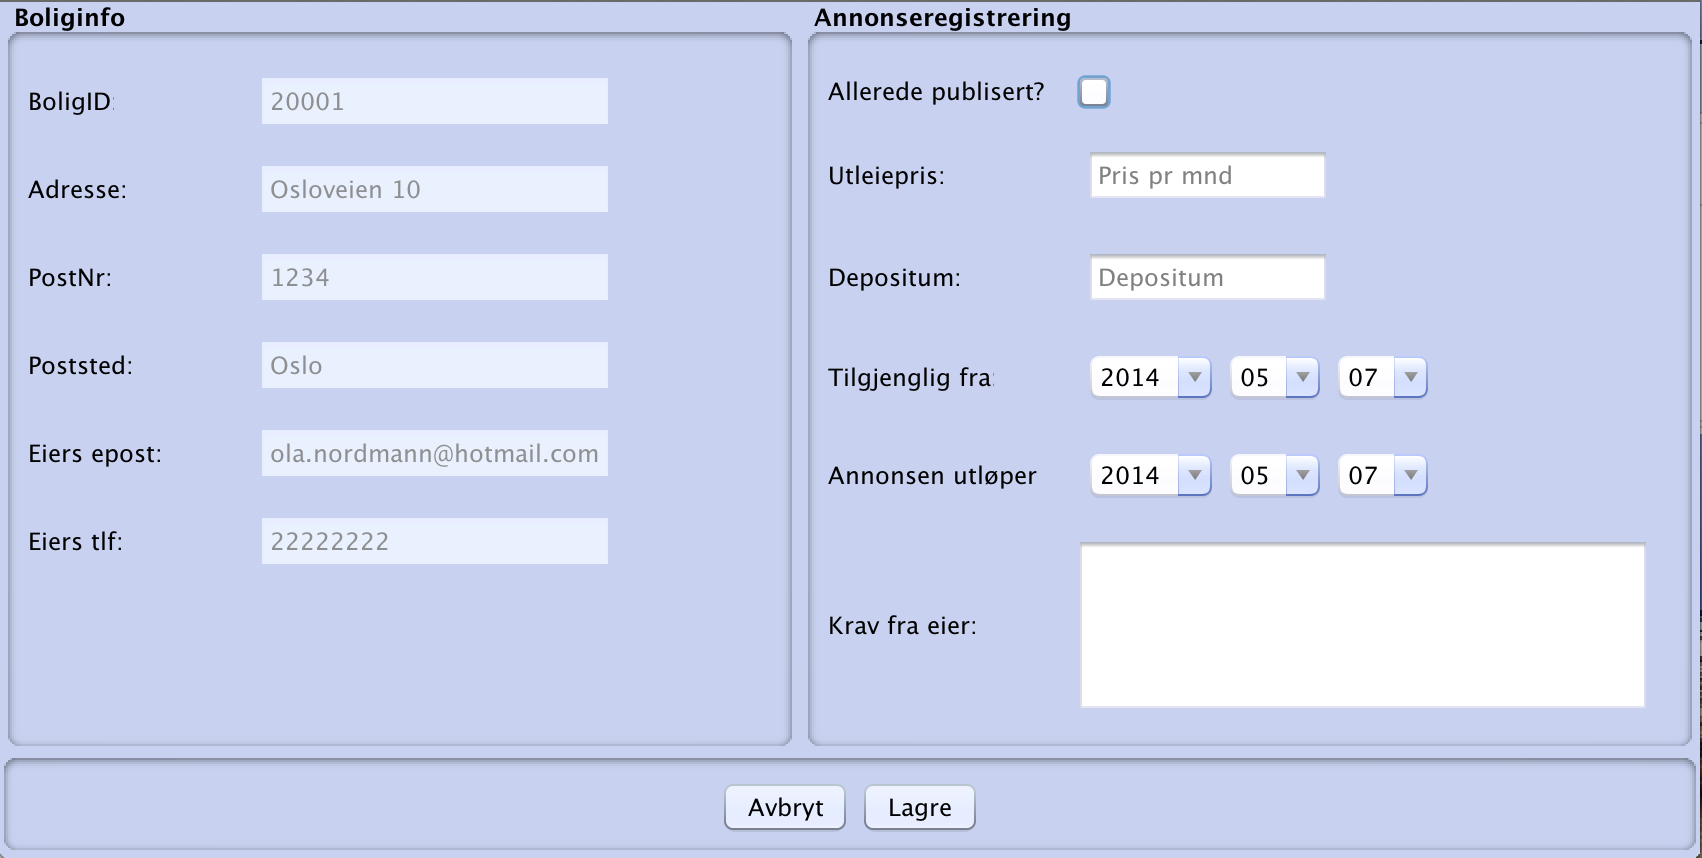
\includegraphics[width=\textwidth,height=\textheight,keepaspectratio]{./img/brukerveiledning/12.png}
 \caption{Annonseadministrasjon.}
 \label{fig:bv:12}
\end{figure}



\newpage
\subsection{Boligadministrasjon}
Ved å søke blant boliger, velge en bolig i listen, og trykke på “Endre” knappen nedest i venstre
hjørne av programvinduet, så har en mulighet til å gjøre endringer i informasjon lagret om boligen,
som vist på figur \ref{fig:bv:13}.

\begin{figure}[h!]
 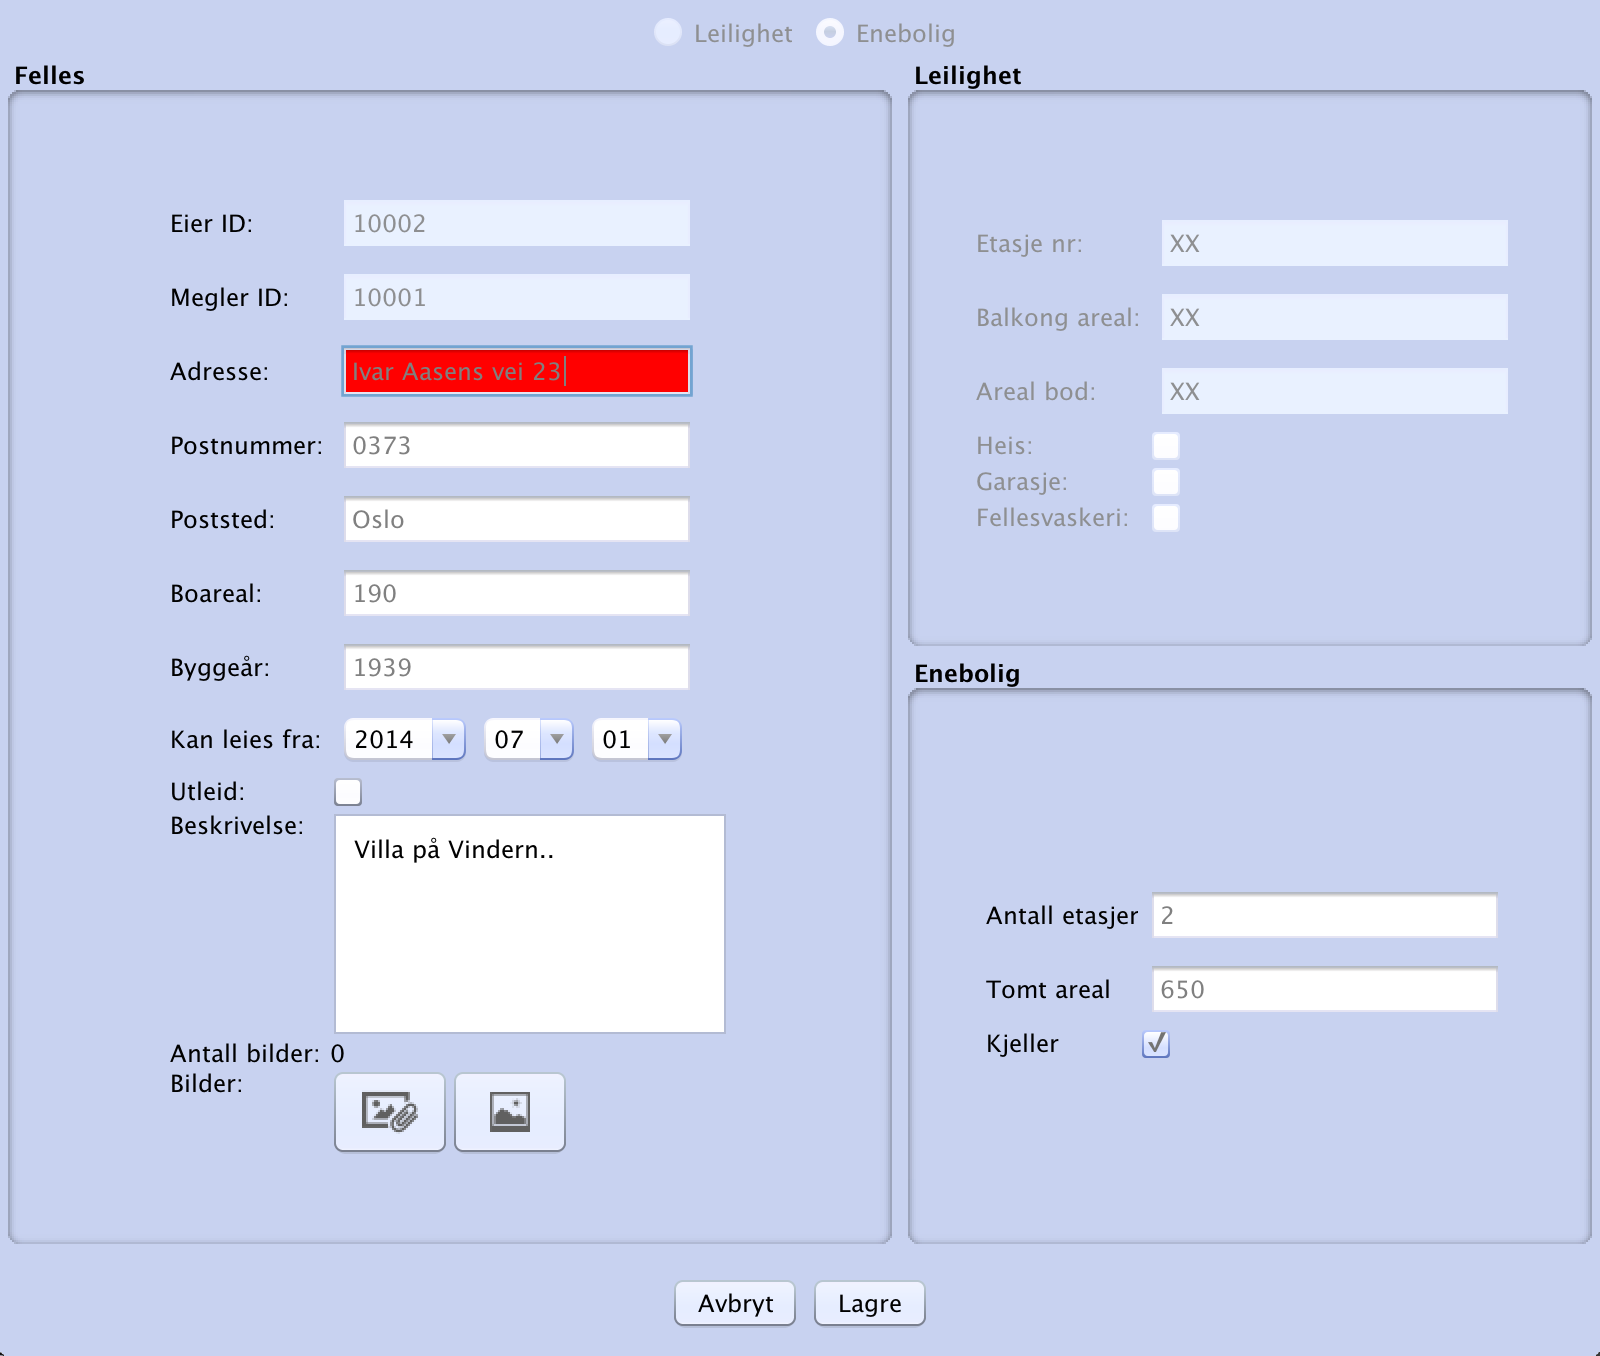
\includegraphics[width=\textwidth,height=\textheight,keepaspectratio]{./img/brukerveiledning/13.png}
 \caption{Boligadministrasjon.}
 \label{fig:bv:13}
\end{figure}


\newpage
\subsection{Kontraktadministrasjon}
Ved å søke etter innkommende søknader, velge en søknad i listen, og trykke på “Ny kontrakt”
knappen øverst i programvinduet, så har en mulighet til å godta, eller avslå den aktuelle søknaden.
Alternativt kan en høyreklikke på den aktuelle søknaden i listen, og velge godta/avslå derfra som
vist på figur \ref{fig:bv:14}. Er det flere søknader på en bolig, så vil de andre bli avslått ved en evnt.
godkjennelse av en søknad.

\begin{figure}[h!]
\center
 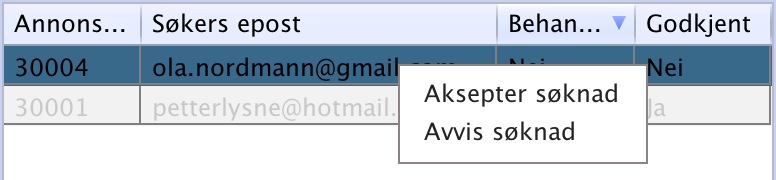
\includegraphics[scale=0.5]{./img/brukerveiledning/14.png}
 \caption{Kontraktadministrasjon.}
 \label{fig:bv:14}
\end{figure}



\subsection{Sletting}
Ved å høyreklikke på et objekt i resultatlisten, så har man mulighet til å slette det valgte objektet.
Alternativt kan “Delete” knappen brukes.

Det er imidlertid noen krav for å få slettet bestemte objekter. Mer spesifikt:

\begin{description}
\item[Slette utleiere] -
En kan ikke slette utleiere med eksisterende registrerte boliger. Boligene må i
såfall slettes først. Boliger som er utleid kan heller ikke slettes før de evnt. ikke lenger er utleid.
\end{description}



\subsection{Hurtigtaster/hotkeys}
For avanserte brukere, så kan hurtigtaster brukes for å oppnå høyere effektivitet, og kjappere
saksbehandling. Følgende hurtigtaster kan brukes:


\textbf{\underline{Generelt}}

\begin{description}
\item[\texttt{CTRL-Tab}] -
Skifter mellom annonse og megler arkfane / tab.
\item[\texttt{Enter/return}] -
Utfører et søk med gjeldende valgte søkekriterier.
\item[\texttt{Pil ned}] -
Blar nedover evnt. søketreff.
\item[\texttt{Pil opp}] -
Blar oppover evnt. søketreff.
\end{description}


